\chapter{Schülerteam: MathePiano Spiel, Login \& Schülerhauptmenü}
Christian Pfeiffer, Normen Krug \& \href{mailto:jofranz90@gmail.com?subject=Swift-Studienarbeit}{Johannes Franz}


\section{Einleitung}
In diesem Abschnitt werden die Ziele und die Motivation des Projektes definiert. Dabei werden unter anderem die Erwartungen an das Projekt genannt.
\subsection{Motivation}
Die Hauptmotivation des Projektes war das Lernen und Einarbeiten in neue Apple Frameworks (wie \textit{SpriteKit} und \textit{CloudKit}) und Erfahrungen sammeln in der Zusammenarbeit mit mehreren Entwicklerteams, welche gleichzeitig an einem Projekt arbeiten. Deshalb war es zwingend notwendig, sich mit anderen Teams zu verständigen und auszutauschen.  

\subsection{Ziele}
Als Ziele der Studienarbeit wurden folgende Punkte definiert: 
\begin{itemize}
\item Kinderfreundliches Design und Layout
\item Erstellen eines Mathelernspieles 
\item Aufgaben die von Lehrern erstellt werden anzeigen und in ein spielbare Form überführen
\item Die von Schüler beantworteten Fragen an den Lehrer weiterleiten
\item Den Schülern die Möglichkeit bieten die Spiele im Endlos Modus, unabhängig der von Lehrer zugewiesenen Aufgaben, zu spielen
\item Lernen eines neuen Apple Frameworks (\textit{SpriteKit})
\item Erfahrung sammeln in Zusammenarbeit mit anderen Teams
\end{itemize}
\section{Spezifikation}


\subsection{Schülerhauptmenü}
\subsubsection{Einleitung}
Primäre Benutzerzielgruppe von Teachify sind Grundschüler. Deswegen ist es wichtig die Hauptmenüs so simpel und zielführend wie möglich zu gestalten. Weiterhin ist es nötig auch die Designsprache so kindgerecht wie möglich zu gestalten.

\subsubsection{Ziele}
\begin{itemize}
    \item Einfache Loginmöglichkeiten
    \item simple Navigationsmöglichkeiten zu Spielen
    \item Unterscheidung zwischen Aufgaben und Endlosspielen
    \item Simple Darstellung von Hintergrundaktivitäten
\end{itemize}

\subsubsection{Einfache Loginmöglichkeiten}
Da es in Teachify zwei Benutzergruppen (Lehrer und Schüler) gibt, muss es eine Möglichkeit geben wie sich diese authentifizieren und danach einloggen können. Als Grundlage unserer App dient das von dem Schnittstellenteam entwickelte "TeachKit". Dies stellt Teachify die von iCloud zur Verfügung gestellten Möglichkeiten zur Verfügung. Zur Authentifizierung des Benuters verwenden wir daher die iCloud Accounts. Innerhalb dieser iCloud Accounts ist aber nicht definiert, ob ein Benutzer zu der Gruppe der Lehrer oder der Schüler gehört. Deswegen wird der Benutzer beim Start von Teachify mit der LoginView begrüßt, innerhalb derer er seine Rolle wählen kann.

\subsubsection{Simple Navigationsmöglichkeiten zu den Spielen}
Nach dem Login als Schüler wird der Benutzer zu dem Schülerhauptmenü weitergeleitet. Innerhalb dessen soll er eine kurze Übersicht über seine Statistiken und bereits erbrachten Erfolgen bekommen. Prominent sollen die Spiele bzw. Übungen welche der Schüler spielen bzw. erarbeiten kann, dargestellt werden. Hierfür sollen die in iOS 11 neu hinzugekommenen Cards dienen, welche ebenso prominent im AppStore verwendet werden. Als weitere Interaktionsmöglichkeiten soll der Schüler in der Lage sein neue Aufgaben aus herunterzuladen und Einladungen, welche in Form von QR-Codes verschickt werden, einzuscannen und somit anzunehmen

\subsubsection{Unterscheidung zwischen Aufgaben und Endlosspielen}
Die Schüler sollen nicht nur in der Lage sein Aufgaben welche von den Lehrern gestellt wurden zu bearbeiten, sondern sollen die implementierten Spiele auch in einen Endlosmodus spielen können. Bei dem Endlosmodus kann der Benutzer endlos lange Aufgaben bearbeiten, welche vorher per Zufallsgenerator generiert wurden. Der Endlosmodus basiert nicht auf von Aufgaben, welche von den Lehrern gestellt wurden.

\subsubsection{Darstellung von Hintergrundaktivitäten}
Da in Teachify oft zeitaufwendige Aufgaben im Hintergrund ausgeführt werden (wie das Abrufen von Daten von der Schnittstelle), muss der Benutzer auch über diese Abläufe informiert werden. Dies soll durch Einblendungen wie einem Progress Indicator, während die Download Operationen laufen, umgesetzt werden.


\subsubsection{User Interface}
\begin{figure}[h]
	\centering
  \frame{ 
  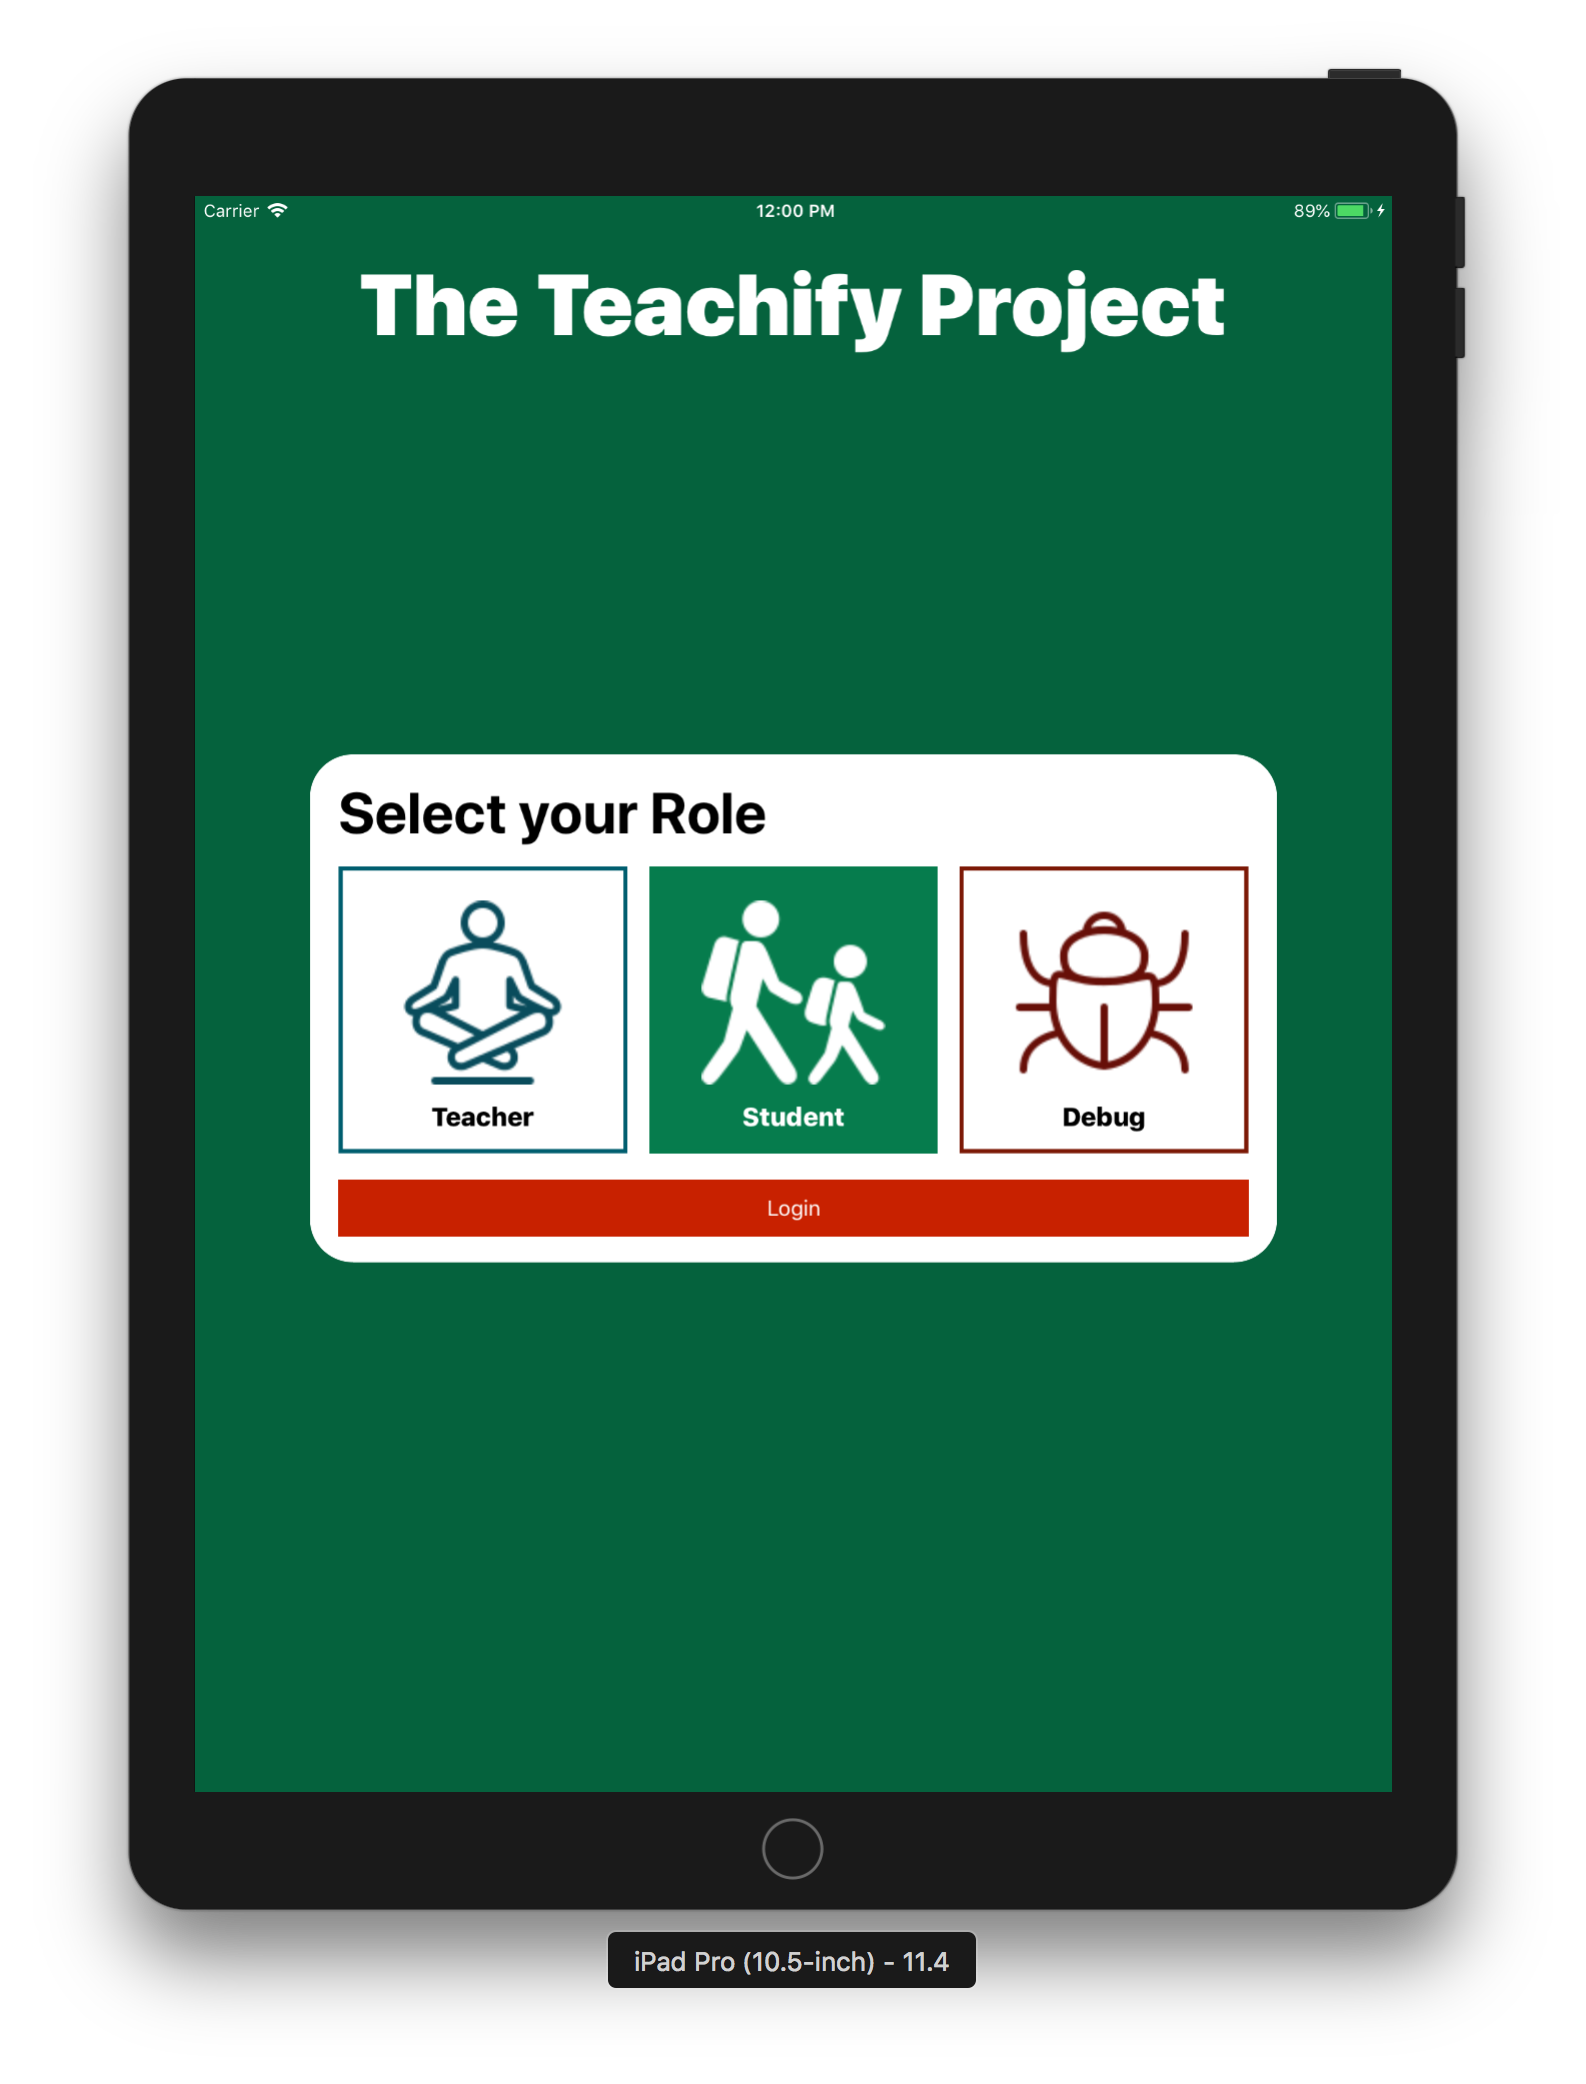
\includegraphics[width=1\textwidth]{images/LoginMenu.png}
  }
	\caption{Der Login Bildschirm (Schüler)}
	\label{Der Login Bildschirm}
\end{figure}

\begin{figure}[H]
	\centering
  \frame{ 
  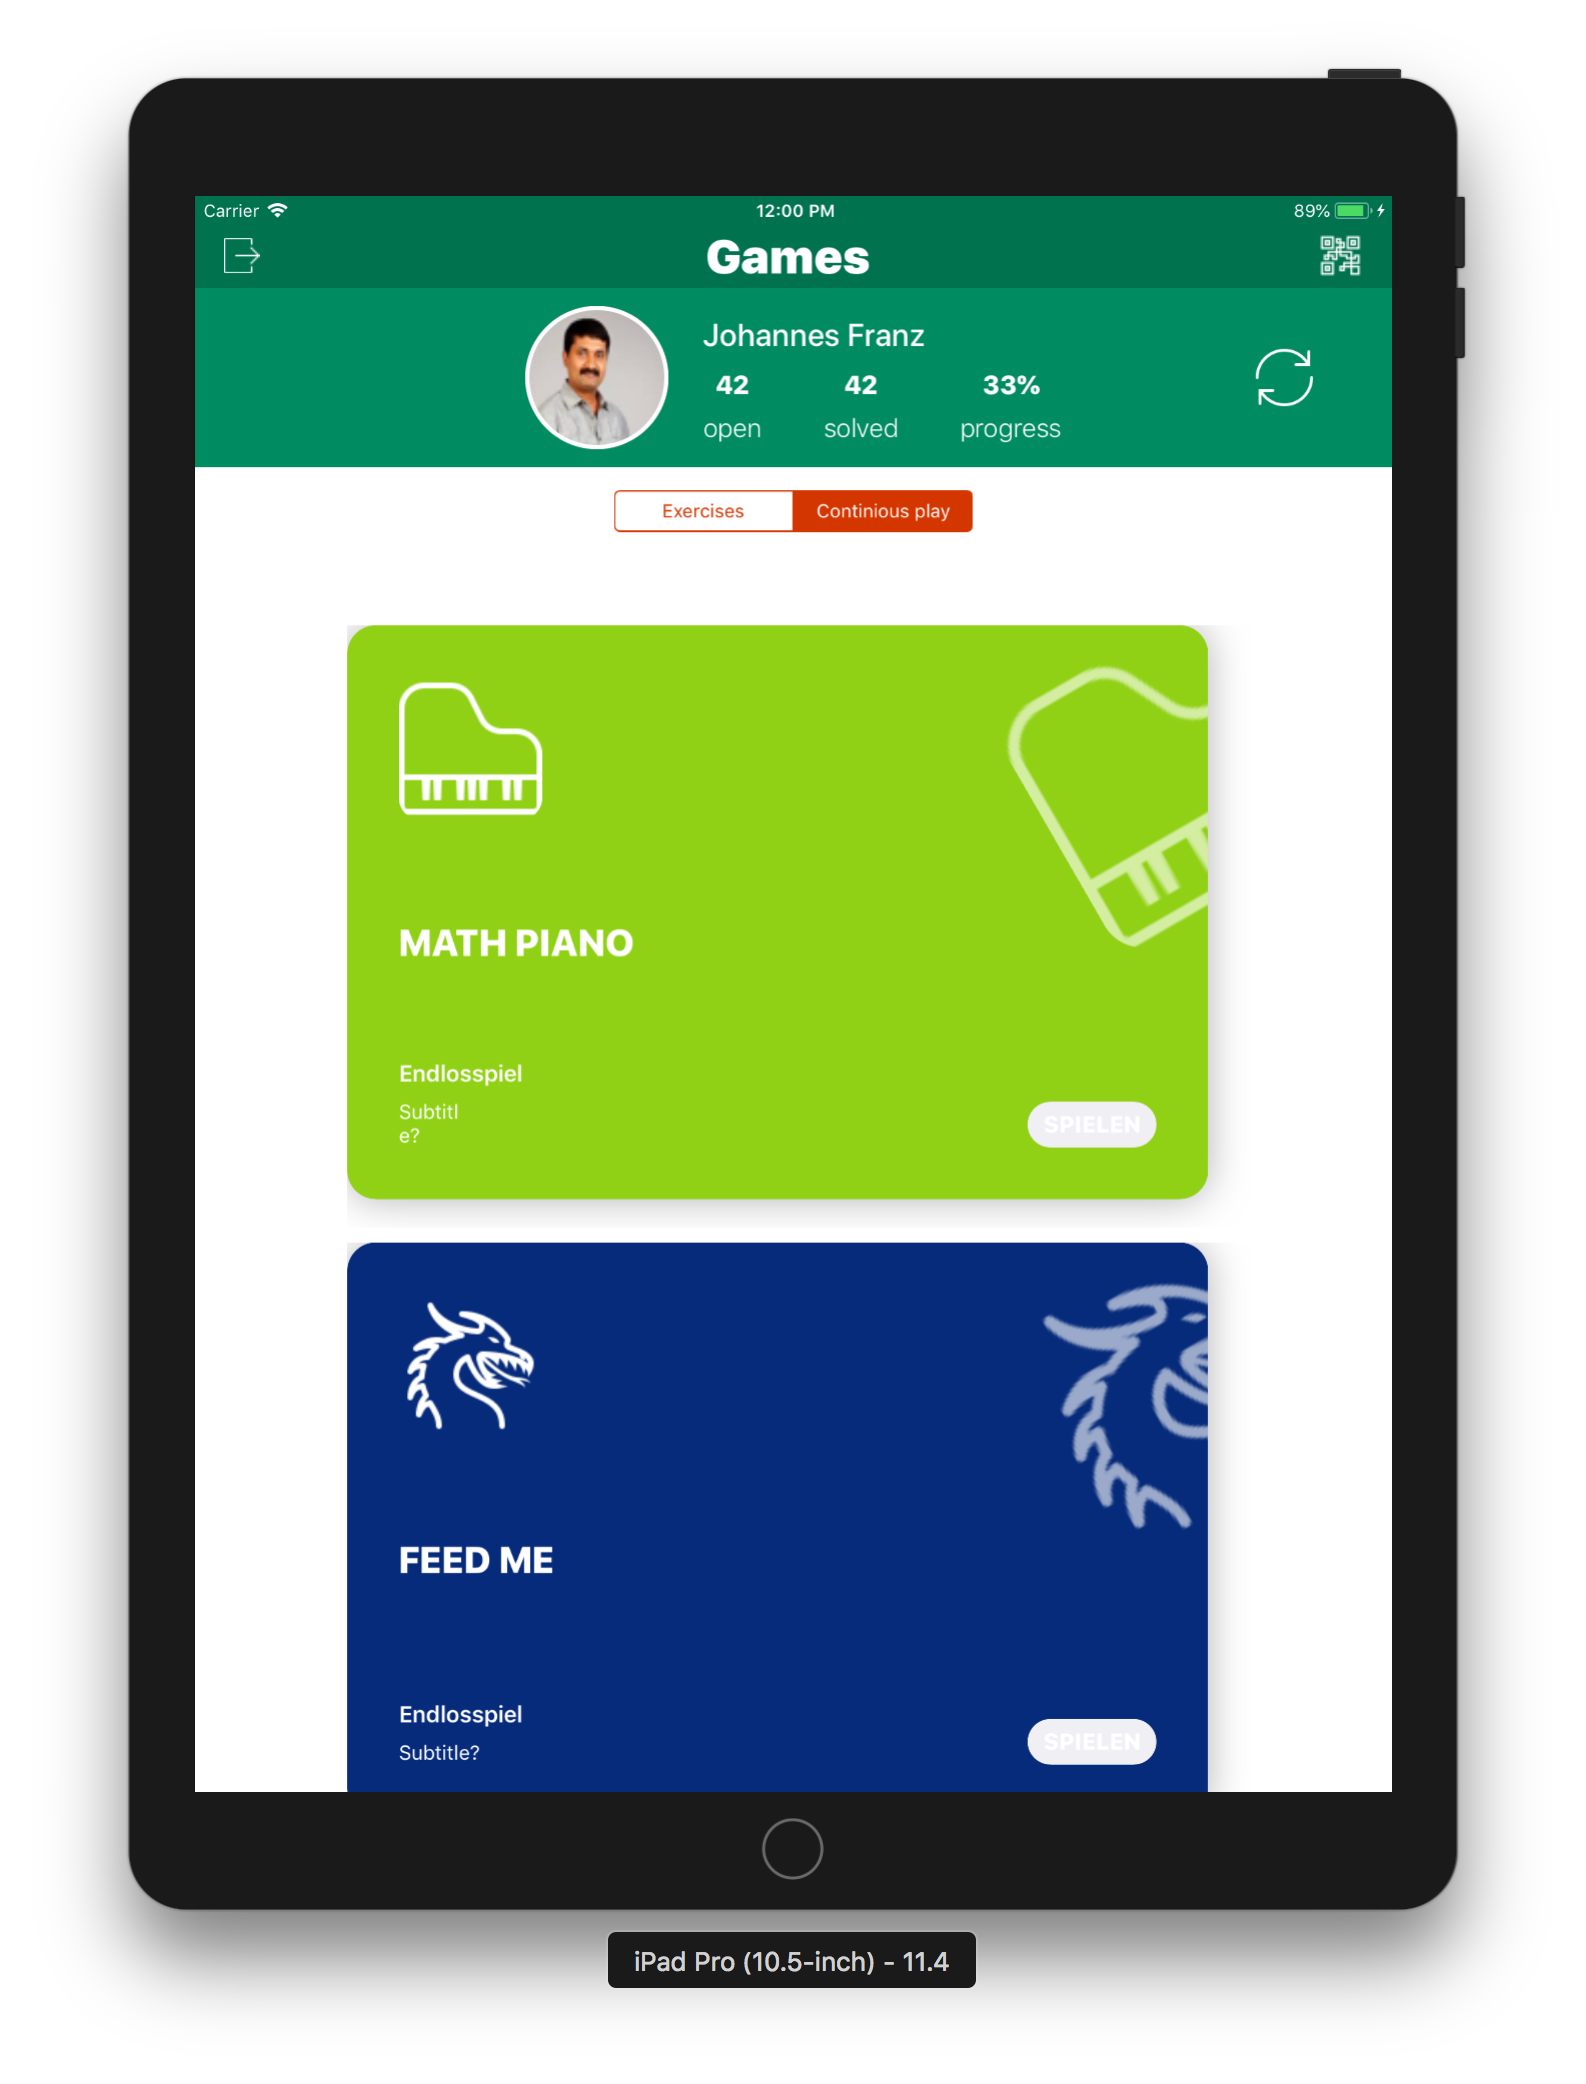
\includegraphics[width=0.99\textwidth]{images/studentMainMenu_Continious.png}
  }
	\caption{Das Schülerhauptmenü (Schüler)}
	\label{Das Schuelerhauptmenue}
\end{figure}
\begin{figure}[H]
	\centering
  \frame{ 
  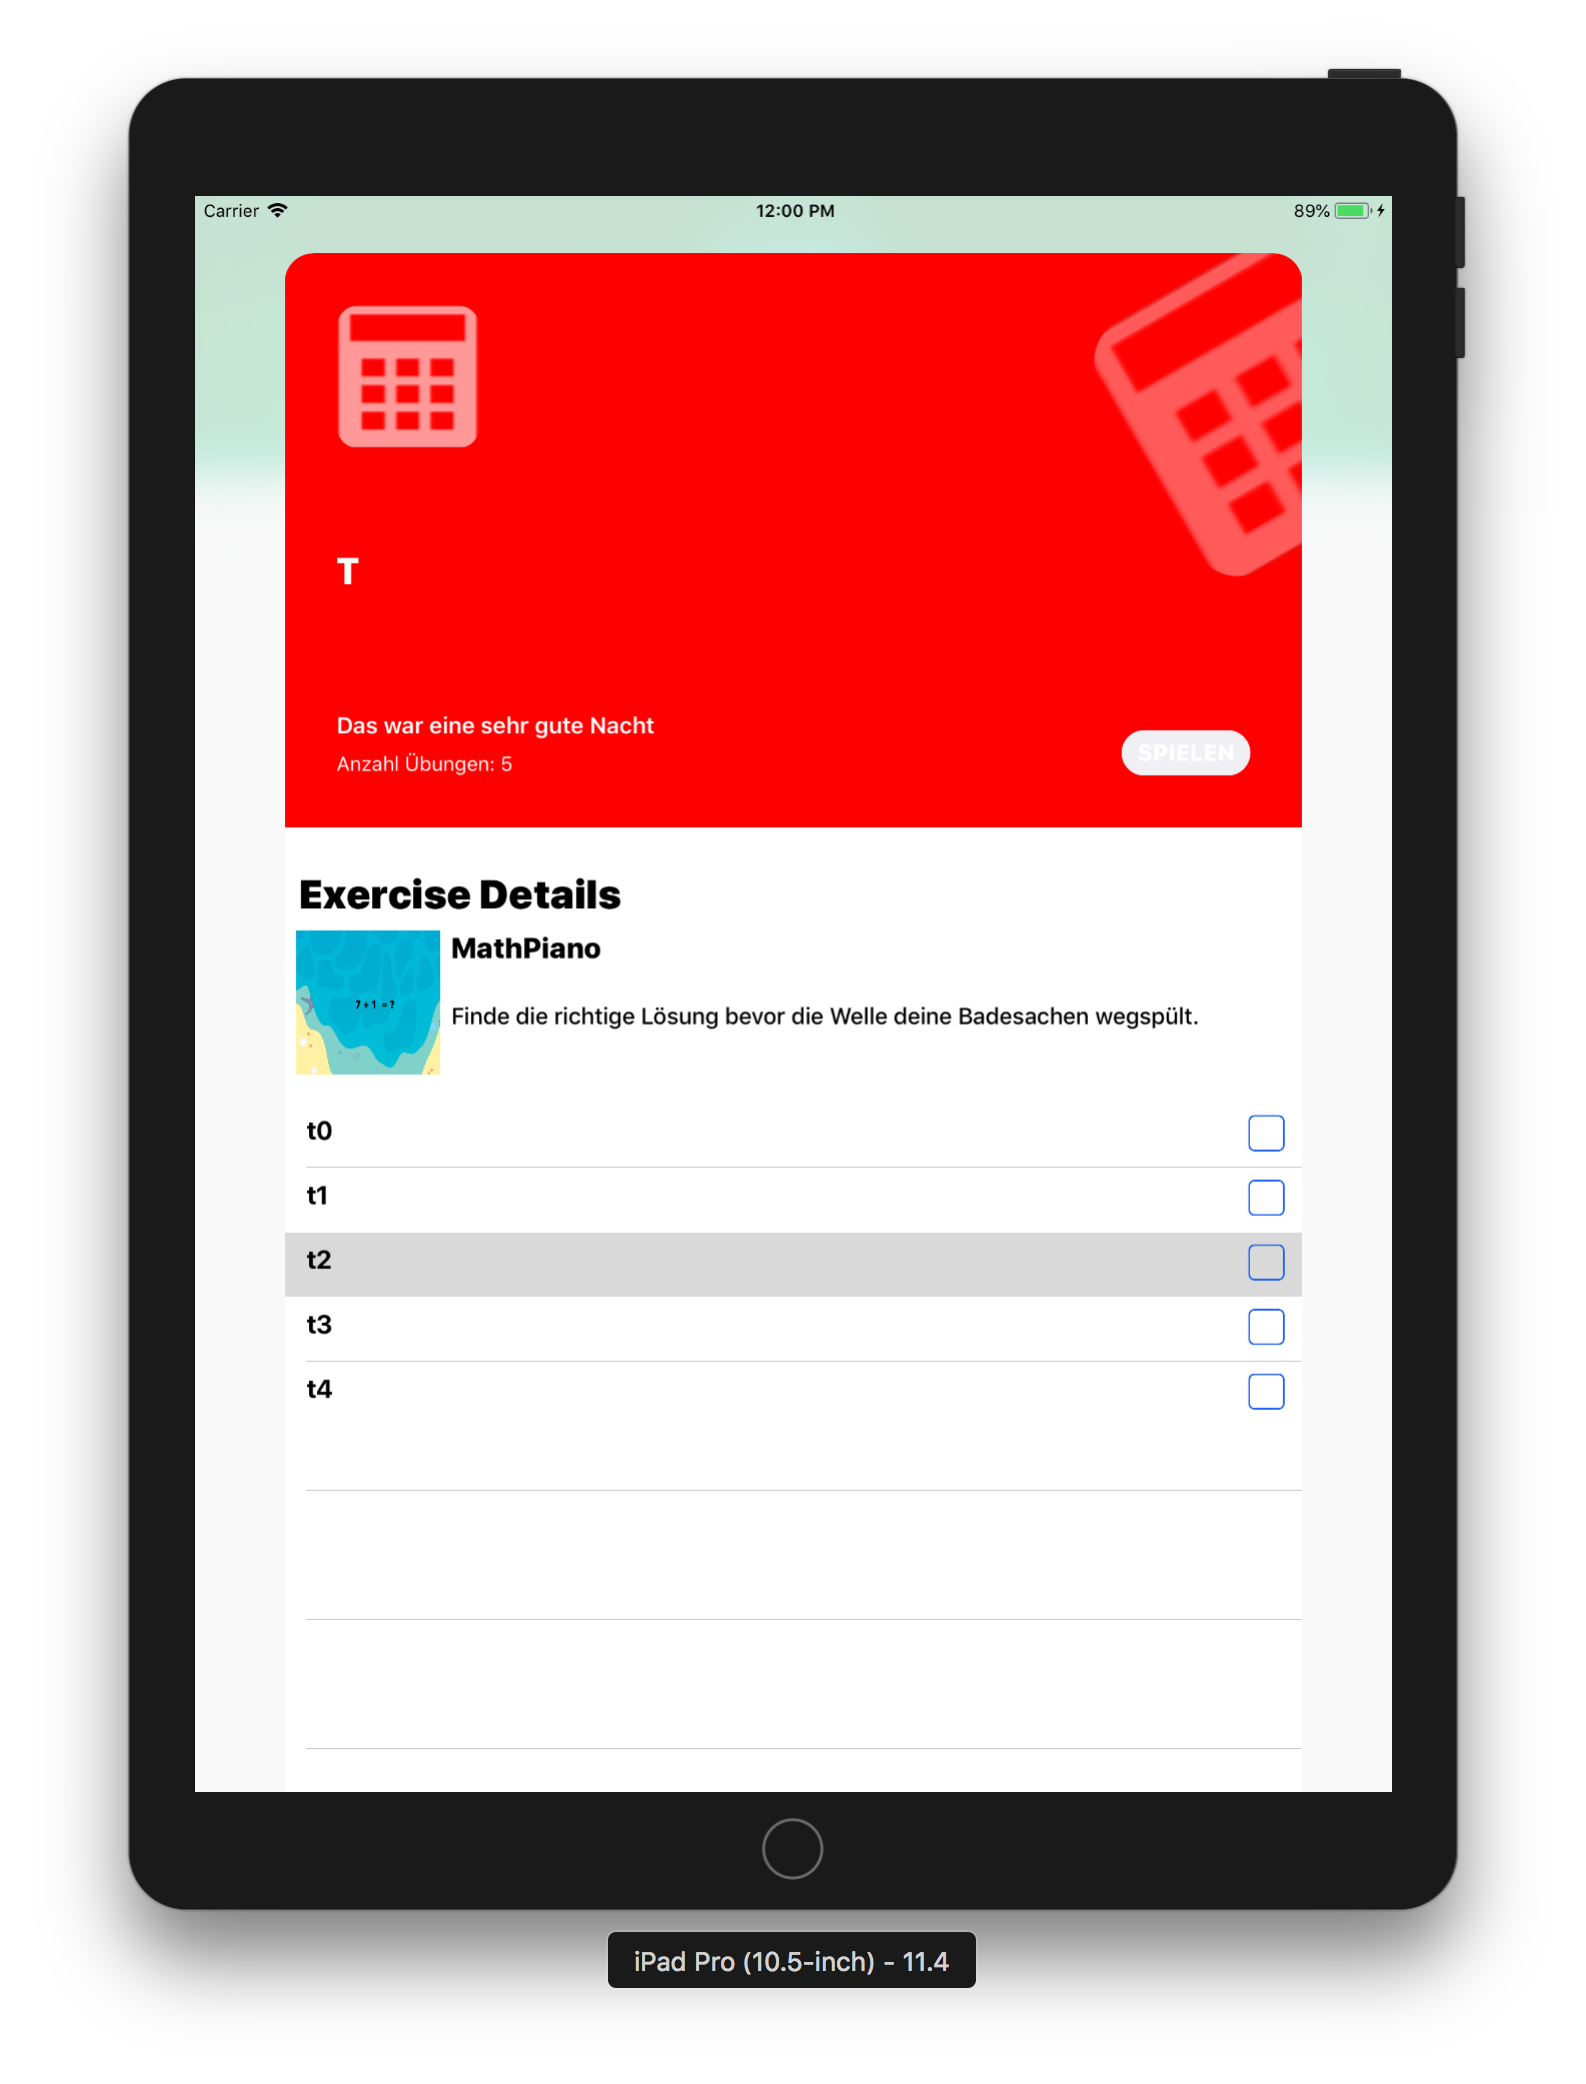
\includegraphics[width=1\textwidth]{images/exerciseDetail.png}
  }
	\caption{Detailansicht einer Übungsaufgabe (Schüler)}
	\label{Detailansicht einer Uebungsaufgabe}
\end{figure}

\subsection{Mathe Piano Spiel}
Bei der Entwicklung des Spiels war es wichtig, möglichst schnell einen funktionsfähigen Prototypen zu ertstellen. Dieser wurde im Verlauf des Projektes immer weiter verbessert.


\subsubsection{Game Engine}
Als Grundlage wurde die von Apple entwickelte Game Engine namens \textit{SpriteKit} verwenden. Diese Engine hat einige Vorteile gegenüber anderen Spielengines:
\begin{itemize}
\item Gute Dokumentation
\item Wiederverwendungen bereits gelernter Paradigmen    
\item Einfache Integrationsmöglichkeit in die App
\item Einfache Anbindung an andere iOS API‘s
\item Swift als Programmiersprache 
\item Schnelles Entwickeln und Testen von Funktionen durch Swift Playgrounds
\end{itemize}

\subsubsection{Herausforderungen}
Nach der ausgiebigen Einarbeitung in das \textit{SpriteKit} \textit{Framework} haben sich einige Hürden ergeben. Das Verwenden von dynamischen Buttons ist nicht trivial, weil es keine Buttons per Default gibt. Deshalb muss eine eigene Button Klasse implementiert und mit der gewünschten Funktionalität erweitert werden. Des Weiteren war es schwierig den Code sinnvoll zu strukturieren, aufgrund der durch Spiel vorgegebenen skriptartigen Programmierung. 
\subsubsection{Testen des Spieles}
Um das Spiel sinnvoll und schon währendes Entwicklungsprozesses testen zu können, musste ein Generator entwickelt werden der zufällige Aufgaben generiert. Dieser befindet sich in der \textit{RandomQuestionGenerator.swift} Klasse. 
\subsubsection{Anbindungen an interne Schnittstellen}
Von Anfang an musste darauf geachtet werden das, dass Spiel an die interne Schnittstelle angebunden werden muss, die von einem anderen Team entwickelt wurde. Da die Schnittstelle nicht von Beginn an verfügbar ist, muss eine temporäre Datenstruktur implementiert werden. Diese soll einfach austauschbar und erweiterbar sein.
\subsubsection{User Interface}
Bei der Gestaltung des User Interfaces muss explizit darauf geachtet werden, dass die Software primär von Kinder bedient wird. Das bedeutet, dass die Größe der Bedienelemente deutlich größer ausfallen muss als bei herkömmlichen Applikationen.   

\section{Implementierungsphase}
An dieser Stelle wird die Implementierung der Aufgaben beschrieben. Dabei wird auf die Schnittstellenanbindung, das Mathe Piano Spiels sowie das User Interface eingegangen.
\subsection{Mathe Piano Spiel}
\subsubsection{SpriteKit}
Durch die Verwendung von den generischen Klassen \textit{BasicNode, BasicButton} konnte schnell auf Änderungen reagiert werden.Besonders zu betrachten ist der \textit{BasicButton}. 
Dieser implementiert das \textit{BasicButtonDelegate}.
\lstinputlisting[language=swift]{source/test.swift}
Mit Hilfe diese Protokolls können Button mit beliebigen Funktionen erstellt werden. 
Alle Nodes werden effizient in der \textit{BasicScene} verwaltet. Die \textit{BasicScene} wird vom \textit{MathPianoGameViewController} erstellt und angezeigt. Wie bei anderen Spielen üblich wird der State der Scene mit jeden neu gerenderten Bild verändert. Dadurch ist es egal auf welchen Device das Spiel läuft.
Schon am Beginn der Implementierungsphase wurde die Software so strukturiert das sie in mehreren Modi gestartet werden kann. Aufgrund des Modi wird der interne State an den jeweiligen Modus angepasst. Diese Modi werden in einen \textit{Enum} abgebildet. Diese hat den Vorteil das es einfach erweiterbar ist, im falle das noch ein neuer Modus dazukommen würde. \\
Die Schwierigkeit des Spiel war es, immer einen konsistenten State zu behalten. Diese war besonders schwierig bei den vielen verschiedenen Iteration Schritten die das Spiele durchlebt hat. Der größte Iterations Schritt war die Vorbereitung auf die Zahlenerkennung. Für diese Feature wurde  parallel eine Testapplikation entwickelt. Bei diesen Prototypen war relativ schnell klar das, dass ausgewählte Modell, aus mehreren Gründen, ungeeignet war. Die Zahlenerkennung funktioniert nicht ausreichend gut, um sie als Ersatz für die \textit{Buttons} zu verwenden. Diese schlechte Erkennungsrate ist auf zwei Hauptfaktoren zurückzuführen.\\
Das Modell wurde mit amerikanischen Zahlen trainiert. Diese unterscheiden sich geringfügig von den deutschen. Durch diese Sprachunterschiede, vorallen bei der Zahl 4,ist die Erkennungsrate messbar schlechter. Der zweite und größere Faktor ist die Art der \textit{Inputschicht} des \textit{neuronale Netzes}.
Das neuronales Netz benötigt Bilder als Eingabequelle.
Die Bilder müssen in einen Format von 28x28 vorliegen. Das hat den entscheidenden Nachteil das man das Bild, welches man aus der \textit{UIView} generiert, stark skalieren muss. Durch diese Skalierung gehen viele Merkmale verloren.
\subsubsection{Game Models}
Der \textit{MathPianoGameViewcontroller} holt sich alle \textit{TKExercises} aus den \textit{TKModelSingelton}, welches in \ref{TKModelSingleton} \nameref{TKModelSingleton} beschrieben ist. Diese \textit{TKExercise} werden in eine Spiel interne Datenstruktur überführt. Das \textit{MathPianoQuestionModel} ist die interne Repräsentation des \textit{TKExercise} nur auf die Anforderung des Spiels optimiert. Die einzelnen \textit{MathPianoQuestionModels} werden im \textit{PianoGame} zusammengefasst. Für diese Umwandlung wurde ein Converter implementiert. 
Im Hintergrund während der Benutzer spielt, werden die Antworten in ein Feedback Model gespeichert. Für diese Aufgabe wurde das \textit{MathPianoGameFeedbackModel} implementiert. \\
Um einen sinnvollen Endlos Spielmodus zu implementieren, werden generierte Fragen benötigt. Für diesen Zweck wurde der \textit{RandomQuestionGenerator} erstellt.

\subsection{User Interface}
\begin{figure}[H]
	\centering
  \frame{ 
  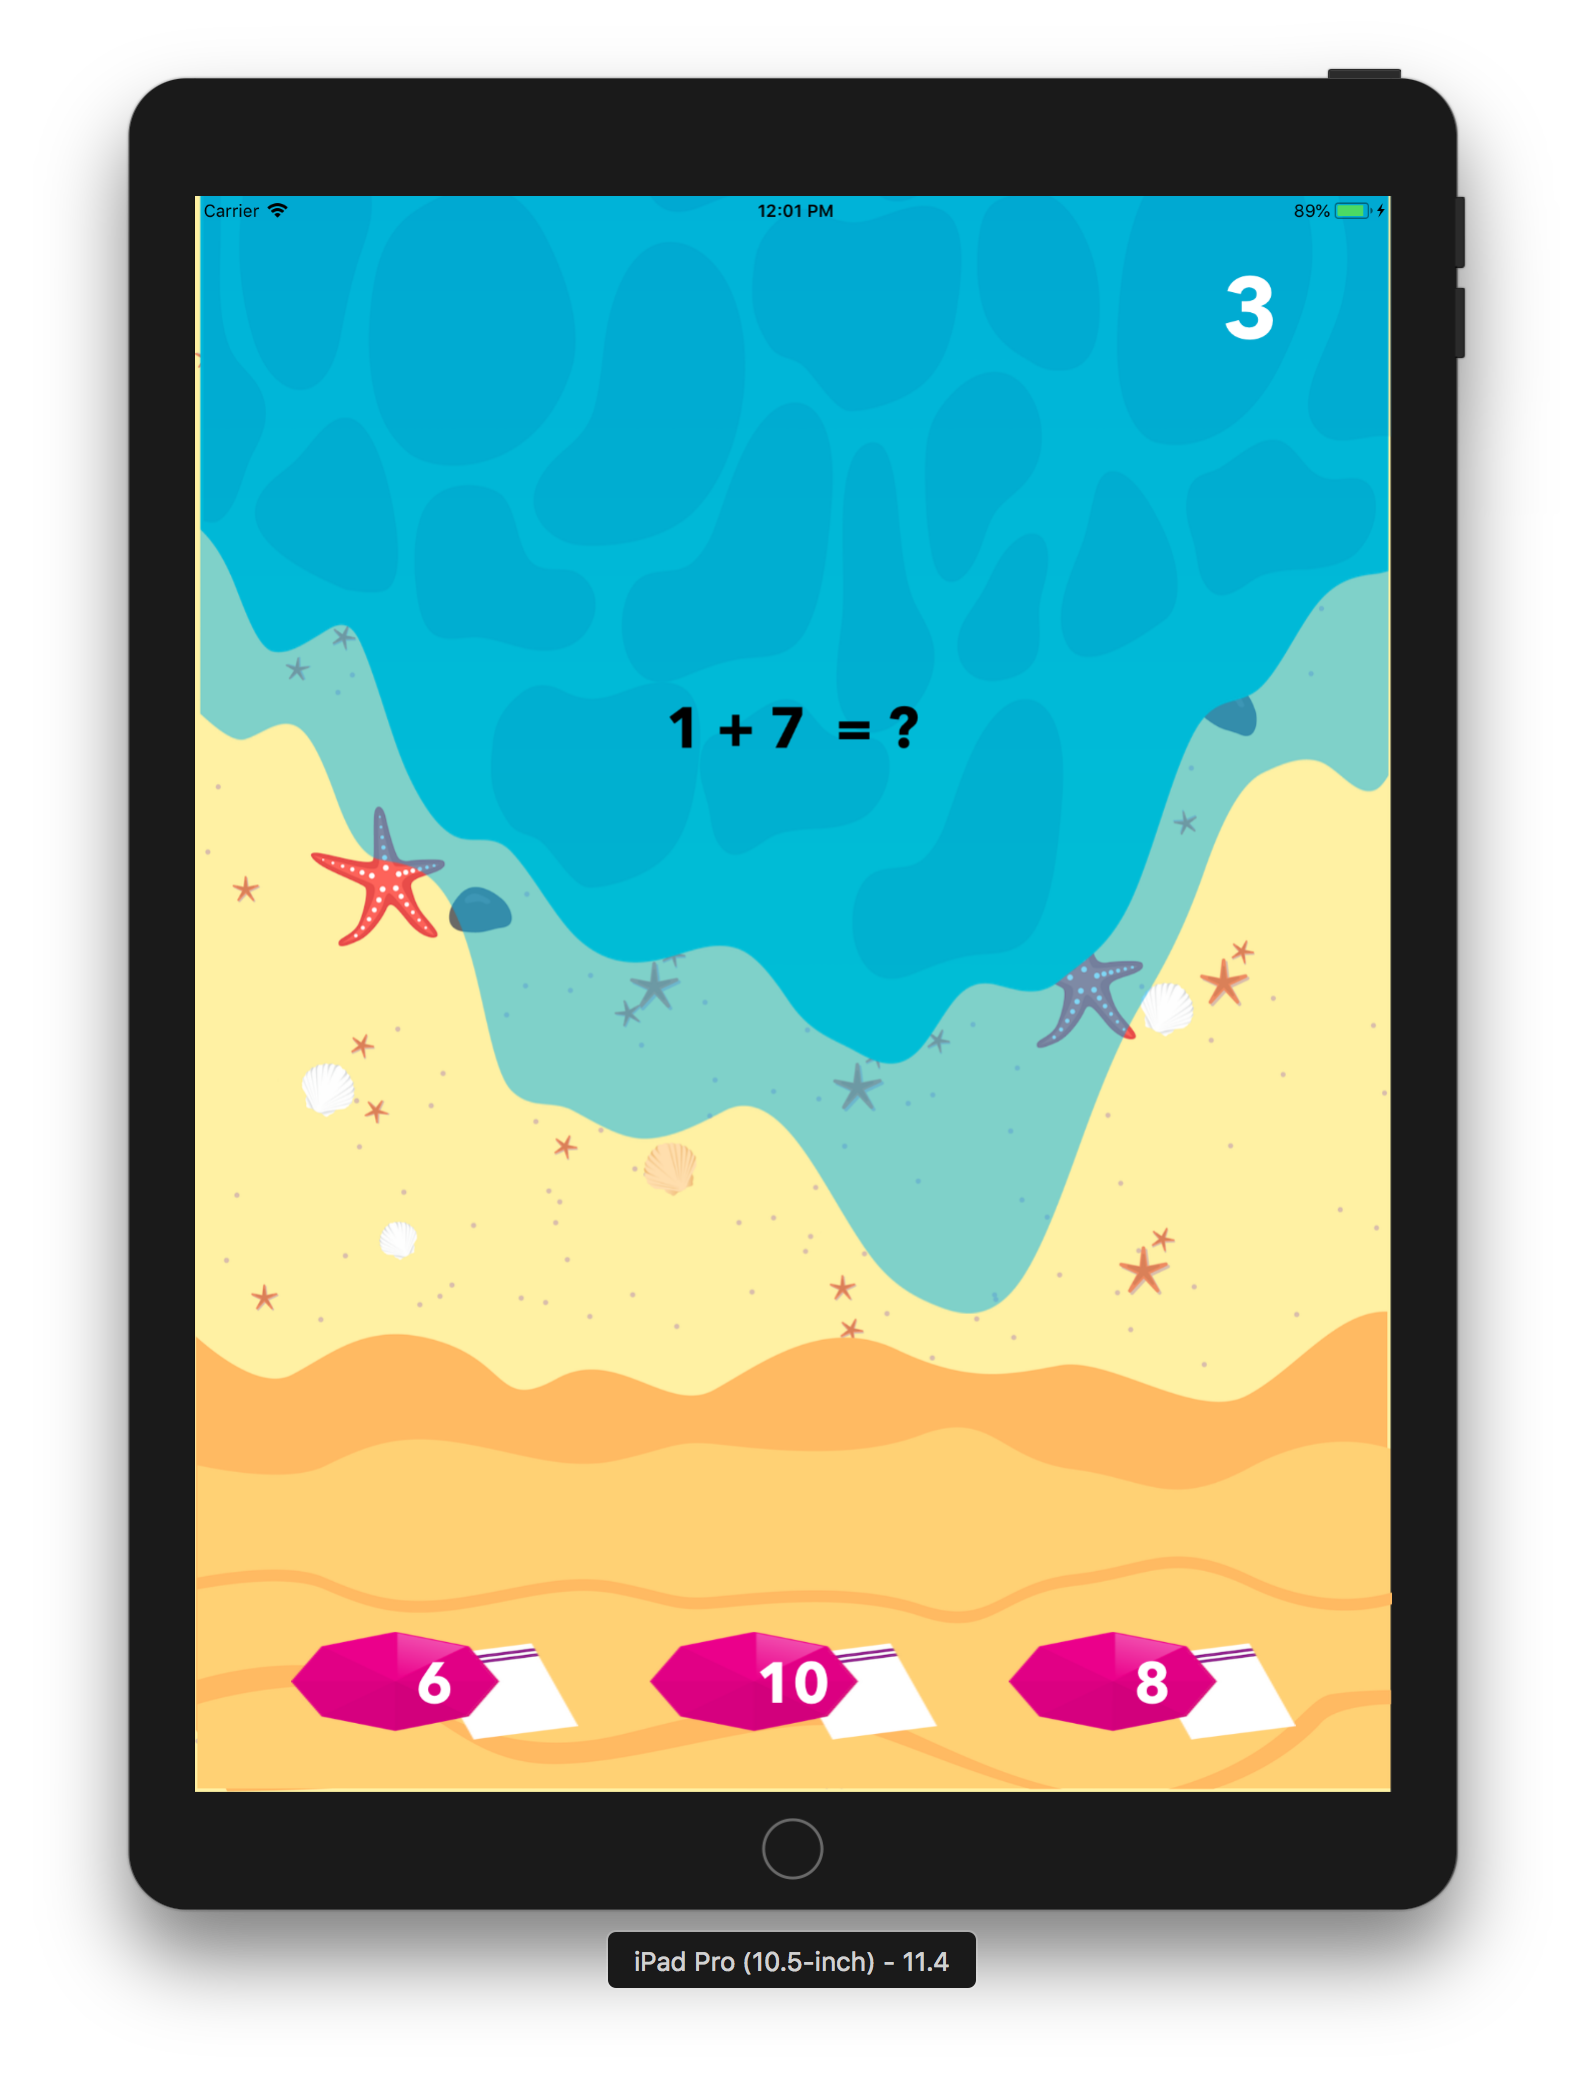
\includegraphics[width=0.5\textwidth]{images/mathPianoGame.png}
  }
	\caption{Das Mathe Piano Spiel}
	\label{Das Mathe Piano Spiel}
\end{figure}
Um das Mathepianospiel so Zielgruppen freundlich wie möglich zu gestalten, wurden verschiedene Grafiken entwickelt, welche ein typisches Strandszenario abbilden. Bei der Farbwahl wurden helle freundliche Farbtöne gewählt. Inhalt des Spiels ist eine Welle, in welcher eine Matheaufgabe abgebildet ist. Der Spieler muss die richtige Antwort auf die Matheaufgabe auswählen, bevor die Welle zu nahe kommt und die Badesachen weg spült.



\section{Fazit}
Teachify war ein herausforderendes Projekt für das 6. Semester. Dies stellte das ganze Team immer wieder vor anspruchsvolle Aufgaben. Der Umgang mit Git (\href{https://github.com/cpfeiffer3008/Teachify}{Teachify Projekt Link}) brachte zugleich viele Vorteile aber auch Herausforderungen.\\
Durch die unterschiedlichen Herangehensweisen (Design vs. Funktion) und den damit weitgehend einhergehenden Verzicht auf einen Prototypen lenkte das Projekt gegen Ende des Projektzeitraums auf einen ``Big-Bang`` Ansatz.
Positiv zu erwähnen war das Zusammenwachsen des Teams und die Zusammenarbeit untereinander. So hatten die meisten Teams eine Domäne in die sie sich eingearbeitet hatten und mussten bei der Überschneidung ihrer Gebiete zusammenarbeiten.